\hypertarget{Approach}{
}
In this section, the data and methods used for the experimental setup are outlined. Because of restricted access to data, only the PhoTex database is available for the experiments. 

\section{PhoTex Database}\label{sec:PhoTex}
The PhoTex database is created for physics-based computer vision. It provides excellent photometric data for texture classification, since all image data is  created under controlled conditions. The materials were recorded under a fixed view and different illumination angles. It also provides the materials under a rotated angle, but these images are discarded for the experiments conducted in this research. The most important features of the database for this research are:
\begin{itemize}
	\item Images are monochromatic.
	\item Resolution: 512 x 512
	\item Fixed and linear gain: images measured under different lighting conditions are comparable. 
\end{itemize}

\noindent The database mainly holds images of rough surfaces, and a few smooth surfaces. For all the image data, the azimuth and zenith angles of the light source are provided (these angles are also mentioned as slant and tilt), making it perfect for photometric stereo algorithms to recover the surface normals and albedo of the materials. The general setup for recording the materials can be seen in figure \ref{fig:PHOTEX_SETUP}. 

The images used in Targhi's experiment are chosen to have a high degree of diffuse reflection properties. All 20 classes are shown in figure X. In order to deal with possible illumination changes of novel data, it is desirable to preprocess the images such that they are intensity invariant by setting the images to zero-mean and unit-variance. 


\begin{figure}[t]
	\begin{center}
		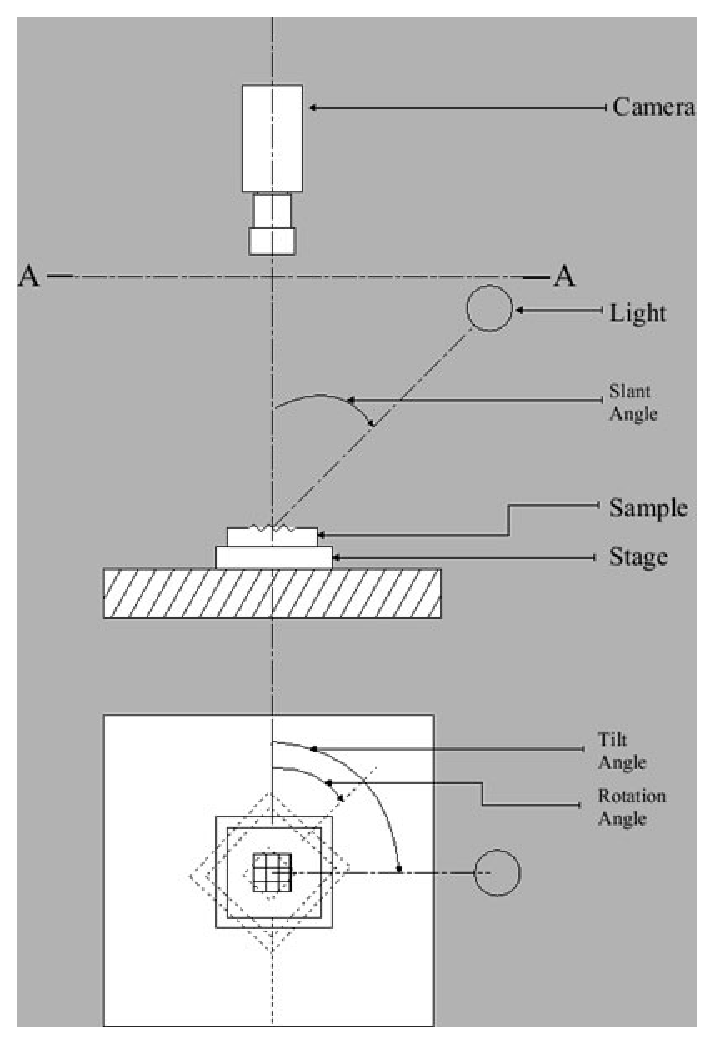
\epsfig{file=images/photex_setup.eps, width=0.5\linewidth}
	\end{center}
	\caption{\textit{Experimental setup of the recording of the PhoTex Database. Courtesy TextureLab @ Heriot-Watt University}}
	\label{fig:PHOTEX_SETUP}
\end{figure}


http://www.macs.hw.ac.uk/texturelab/

\section{Photometric Stereo}\label{sec:PhotometricStereo}
The aim of photometric stereo is to estimate at every point of a given object the albedo and surface normal. This is done by using a set of images of this object under different illumination conditions. 

The viewpoint is assumed to be perpendicular to the surface patch that needs to be recovered, and the source light illuminating the surface patch is assumed to be a point light (\textit{eg.} the source is positioned at an infinite distance with as a result give an equal angle of incidence for all points on the surface patch). Using the Lambertian reflection model and assuming there is no global illumination present in the data, the radiosity \textbf{B} at a point $(x, y)$ on the surface can be written as:

	\begin{eqnarray*}
		\textbf{B}(x,y) = \rho(x,y)\textbf{N}(x,y) \cdot \textbf{V}
	\end{eqnarray*}

With $\rho(x,y)$ the albedo at point $(x,y)$, $\textbf{N}(x,y)$ being the surface normal at point $(x,y)$ and $\textbf{V}$ being the source light vector. Both the surface normal and source light vector are unit in length. With the assumption that the camera response is linear to the surface radiosity, the value for a pixel at point $(x,y)$ in the image is equal to the radiance at that point. The above equation can be written as:

	\begin{eqnarray*}
		I(x,y) =  \textbf{g}(x,y) \cdot \textbf{V}
	\end{eqnarray*}
Where $\textbf{g}(x,y)$ is equal to $\rho(x,y)\textbf{N}(x,y)$ and describes the properties of the surface we want to recover. Given that $\textbf{V}$ is known for the image data, with enough dot products between $\textbf{g}(x,y)$ and $\textbf{V}$, the values for $s\textbf{g}$ could be recovered. With known values for $\textbf{g}$, the albedo and surface normals in turn could be recovered.

If we have $n$ images all recorded under the same viewing angle with $n$ different light sources with known light source direction, we can construct a matrix where all values $V_i$ are stacked on each other:

	\begin{eqnarray*}
		\textbf{V} = \begin{pmatrix} V_1^T \\ V_2^T \\ ... \\ V_n^T \end{pmatrix}
	\end{eqnarray*}



\section{Classification}\label{sec:Classification}
\begin{itemize}
	\item{multivariate Gaussian Classifier, Mallow distance}
\end{itemize}

\section{Reflection Models}\label{sec:ReflectionModels}
	In previous work on image synthesis done by Targhi as described in section \ref{sec:Minimal}, the synthetic data is being created using the Lambertian reflection model. This model includes self-shadows and diffuse reflection, but no specularity or interreflections. In this research, the application of more complex reflection models is studied...

